\section{Setup}
In order to evaluate the performance of \ac{CORN} in \dsea{},
a dataset has to be prepared
and hyperparameters need to be chosen.
%
The setup is largely based on previous works
  \cite{dsea_jan, dsea_samuel}
to ensure comparability of the results
  as much as possible.


\subsection{Monte Carlo Dataset and Preprocessing}
% █ Monte Carlo dataset
%
% NOTE: Full description from the website
% Level2 w/systematics IC86.2012 neutrino-generator NuMu with weighted spectrum of E^-2, using SpiceLea CLSim.
% Angular range of 0. deg < theta < 180. deg and energy range of 1e2 GeV < Enu < 1e8 GeV.
%
The unmodified dataset \emph{11374} \cite{icecube_mc} consists of about 13 million Monte Carlo simulated
  \hyperref[sec:neutrino_astronomy:icecube:up_going]{up-going}
  muon neutrino events,
% NOTE: Exact number is 13336413 before any preprocessing.
with a weighted $E^{-2}$ energy spectrum
ranging from \SI{E2}{\giga\electronvolt} to \SI{E8}{\giga\electronvolt}.
The energies are stored under the key \texttt{MCPrimary.energy}.
See \autoref{fig:dataset:raw:histogram} for a histogram of the data.
% NOTE: Jan claims the number of features to be 79,
% but subtracting the index and 4 MCPrimary keys gives me 99-1-4=94

To ensure comparability to \cite{dsea_jan} and \cite{dsea_samuel}, % COULDDO: already cited in intro
only the first \num{500000} events of the dataset are considered.
This also allows for more thorough hyperparameter optimization,
which would otherwise be limited by
  the available computational resources
  as well as the timeframe of this thesis.
% COULDDO: The smallest bin contains approximately XY events.
%
Unless otherwise stated, % NOTE: ≙ Whenever I don't use bootstrapping
\SI{90}{\percent} of the data is used for training,
while the remaining \SI{10}{\percent} is used for evaluation.
No separate validation set is used.


% █ Feature Selection
Because
  unfolding is highly dependent on the selection of features \cite{dsea_jan} % COULDDO: find a better reference
  and training is negatively affected by the presence of irrelevant ones \cite{dash1997},
not all available features are considered.
%
\citeauthor{dsea_jan} \cite{dsea_jan} has employed the \emph{mRMR} (Minimum Redundancy Maximum Relevance) algorithm \cite{mrmr}
to select the 12 most relevant features.
The algorithm takes into account both
  the \emph{relevance} of a feature to the target variable,
    measured by their correlation,
  and the \emph{redundancy} of a feature to other features.
This way,
the \emph{minimal-optimal} set of features is selected,
  in contrast to the \emph{all-relevant} set of features,
    which would also contain redundant features \citationneeded{}. % Spoiler alert: I can't find a citation for this.
    % which would be selected by a simple relevance-based feature selection algorithm. % Copilot blah blah
A list of said features is provided in \autoref{tab:features_best}.
They are reused in this thesis.

\begin{table}
  \centering
  \begin{tabular}{l}
    \toprule
    % \midrule
    % NOTE: MCPrimary.energy is excluded
    \texttt{SplineMPEDirectHitsICE.n\_dir\_doms} \\
    \texttt{VariousVariables.Cone\_Angle} \\
    \texttt{SplineMPECramerRaoParams.variance\_theta} \\
    \texttt{Borderness.Q\_ratio\_in\_border} \\
    \texttt{SplineMPETruncatedEnergy\_SPICEMie\_BINS\_MuEres.value} \\
    \texttt{SplineMPETruncatedEnergy\_SPICEMie\_DOMS\_Neutrino.energy} \\
    \texttt{SplineMPEDirectHitsICB.n\_late\_doms} \\
    \texttt{Dustyness.n\_doms\_in\_dust} \\
    \texttt{LineFitGeoSplit1Params.n\_hits} \\
    \texttt{SplineMPEDirectHitsICC.dir\_track\_hit\_distribution\_smoothness} \\
    \texttt{SPEFit2GeoSplit1BayesianFitParams.logl} \\
    \texttt{SplineMPECharacteristicsIC.avg\_dom\_dist\_q\_tot\_dom} \\
    \bottomrule
  \end{tabular}
  \caption{
    12 best features according to the \emph{mRMR} algorithm \cite{dsea_jan}.
  }
  \label{tab:features_best}
\end{table}


% █ Transformation
It has been shown that none of the selected features are normally distributed \cite{dsea_jan}.
In accordance with \cite{dsea_jan},
the features are therefore transformed using the \emph{Yeo-Johnson} transformation \cite{yeo_johnson},
a power transformation which reduces skewness.
% https://en.wikipedia.org/wiki/Power_transform#Yeo–Johnson_transformation
% NOTE: Positive effect on OUR performance is unverified.
%
Additionally, zero-mean, unit-variance normalization is applied to all features.
% TODO: Expand on this.


% █ Discretization
As described in \autoref{sec:dsea:dsea}, \dsea{} requires discrete energy classes.
The target variable \texttt{MCPrimary.energy} is therefore discretized into \num{10} bins
(in accordance with \cite{dsea_samuel}).
%
Contrary to \cite{dsea_jan} and \cite{dsea_samuel},
under- and overflow bins are added
  in order to allow for the application to real data.
%
The lower limit of the overflow bin is chosen so that it contains a similar number of events as the previous bin,
ensuring sufficient statistics.
A lower energy limit of \SI{E5}{\giga\electronvolt} (in accordance with \cite{dsea_samuel}) was found to satisfy this requirement.
%
The underflow bin is assigned the energy range from \SI{E2}{\giga\electronvolt} to $10^{2.1} \si{\giga\electronvolt}$
  because the dataset does not contain any events with exceptionally low energies below \SI{E2}{\giga\electronvolt}.
This way, the event count in the underflow bin is similar to the neighboring bin.
%
The remaining \num{8} bins are spaced logarithmically between the under- and overflow bins
  so that the entire energy range of the Monte Carlo dataset is covered.
%
A histogram utilizing the aforementioned bins is shown in \autoref{fig:dataset:discretized:histogram}.

\begin{figure}
  \centering
  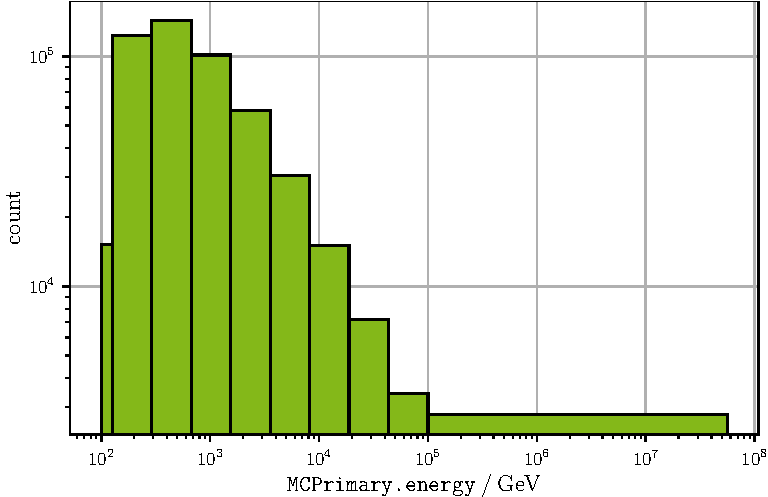
\includegraphics[scale=1]{content/plots/dataset_500k:discretized:histogram_full.pdf}
  \caption{Energy spectrum of the 500k Monte Carlo dataset using the discretized energy ranges as bins.}
  \label{fig:dataset:discretized:histogram}
\end{figure}


\subsection{Neural Network and \dseatitle{}}
% █ Neural network
A PyTorch \cite{pytorch} implementation of the \ac{CORN} method
as well as several examples demonstrating its application on different datasets
is provided by \cite{corn}.
% NOTE: https://raschka-research-group.github.io/coral-pytorch/tutorials/pytorch_lightning/ordinal-corn_cement/
%
This work makes use of said implementation of \ac{CORN}
and hence the PyTorch framework.
Additionally,
  PyTorch Lightning \cite{pytorch_lightning},
  TorchMetrics \cite{torch_metrics}, % Oxford comma
  and scikit-learn \cite{sklearn}
  are used.

The neural network consists of \num{4} fully connected hidden layers.
The input layer has \num{12} neurons,
  corresponding to the number of features,
while the output layer has \num{9} neurons,
  corresponding to the number of binary classification subtasks,
    i.e. the number of bins minus one.
In total,
the neural network has about \num{6100} trainable parameters.
%
  The number of neurons
  and the activation function
per layer
are shown in \autoref{tab:nn_shape}.
%
In order to retrieve probabilities from the output neurons,
  a modified version of the \ac{CORN}-provided function \mintinline{python}{corn_label_from_logits(logits)} is used,
    which implements the conversion
      from threshold- to per-class probabilities
    outlined in \autoref{sec:ordinal:corn:probas}.


\begin{table}
  \centering
  \begin{tabular}{S[table-format=3.0] c}
    \toprule
    {neurons} & {activation function} \\
    \midrule
     12 & – \\
    120 & leaky ReLU \\
    240 & leaky ReLU \\
    120 & leaky ReLU \\
     12 & leaky ReLU \\
      9 & leaky ReLU \\
    \bottomrule
  \end{tabular}
  \caption{
    Shape and activation functions of the neural network.
    The number of neurons in the input and output layers is determined by the number of features and bins, respectively.
  }
  \label{tab:nn_shape}
\end{table}

\ac{Adam} \cite{adam} is used as the optimizer.
% It combines the benefits of both AdaGrad and RMSProp.
It minimizes the loss function provided by \ac{CORN} (see \autoref{eqn:corn:loss}).

The neural network keeps its weights between \dsea{} iterations.
In theory,
  this could improve its performance,
    analogous to \emph{fine-tuning} a pre-trained model.
However,
\cite{dsea_samuel}
% demonstrated that the approach has
found
no significant effect on the performance.
% NOTE: → one_model


% █ DSEA
For this work, the Python implementation of \dsea{} \cite{dsea_code} is used,
  which expects a \emph{scikit-learn} classifier.
In order to interface with this library,
a wrapper class is implemented,
  which exposes a constructor as well as the needed methods
  \mintinline{python}{fit(X, y, sample_weight)} and
  \mintinline{python}{predict_proba(X)}.

\smallskip % COULDDO: Hack to prevent page break
% \FloatBarrier
